\subsection{Gaussian Beam Propagation and Fraunhofer Diffraction}
	\label{diffraction}
	
The far-field light field is the Fourier transform of the aperatured field.
	
\begin{equation} 
E(k_{x},k_{y}) = \mathcal{F}\left\{{\overbrace{t(x,y)}^{Aperature\  transmission\  function}\cdot E(x,y)}\right\} = \iint(exp(-i(k_{x} x + k_{y}y))\cdot t(x,y)\cdot E(x,y)dxdy 
\end{equation} 

Gaussian Fourier Transform

\begin{equation} 
\mathcal{F}\left\{{\overbrace{exp \frac{-(x^{2} + y^{2})}{w^{2}_{0}}}^{Gaussian\ radial\ profile}} \right\} \propto\left[\frac{-(k_{x},k_{y})\cdot w^{2}_{0}}{4}\right]
\end{equation}

\begin{figure} [ht]
\centering
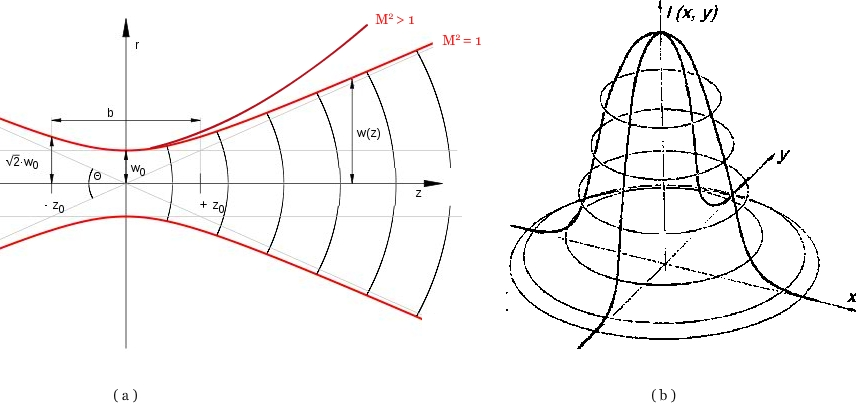
\includegraphics[scale=0.5]{chapters/img/TEM00.jpg}	
\caption{Transverse Mode}
\label{laser_power}
\end{figure}

w1 equals

\begin{equation}
w_{1} = \frac{\lambda \cdot z}{\pi\cdot w_{0}}
\end{equation}
\

theta equals

\begin{equation}
\theta = \frac{\lambda}{\pi\cdot w_{0}}
\end{equation}
\

